\chapter{Anforderung an die Migration einer Anwendung}
\label{chap:anforderungen}

Das nachfolgende Kapitel befasst sich mit den funktionalen und nicht-funktionalen \mbox{Anforderungen}, die an die migrierte Anwendung gestellt werden. Funktionale Anforderungen umfassen hierbei den Funktionsumfang, also zum Beispiel Prozessabläufe, wogegen nicht-funktionale Anforderungen sich auf die Ausnutzung der Vorteile durch die Cloud fokussieren.

% Anforderungsanalyse
\section{Anforderungsanalyse}

Um ein Migrationskonzept entwerfen zu können wird zuerst die existierenden Anwendung kurz beschrieben und untersucht und mithilfe einer Literaturrecherche die notwendigen Anforderungen an die Migration erarbeitet.

\subsection{Existierender Code}
Ziel der Anwendung ist das Einsammeln der Timesheets, in dem Projekt aktiver Mitarbeiter, aus einem Box Verzeichnis, das Überprüfen dieser und die anschließende Rechnungs- und Report Erstellung. Die Prozesse werden jeweils manuell über eine Konsoleneingabe gestartet. Im Box-Verzeichnis liegt ein Projektmanagement-File, welcher alle Mitarbeiter enthält, die jemals in dem Projekt gearbeitet haben und markiert, welche auch aktuell aktiv sind und dem Kunden in Rechnung gestellt werden können. In Abbildung \ref{fig:pmo_python} wird der Aufbau der ursprünglichen Anwendung dargestellt.

\begin{figure}[H]
    \centering
    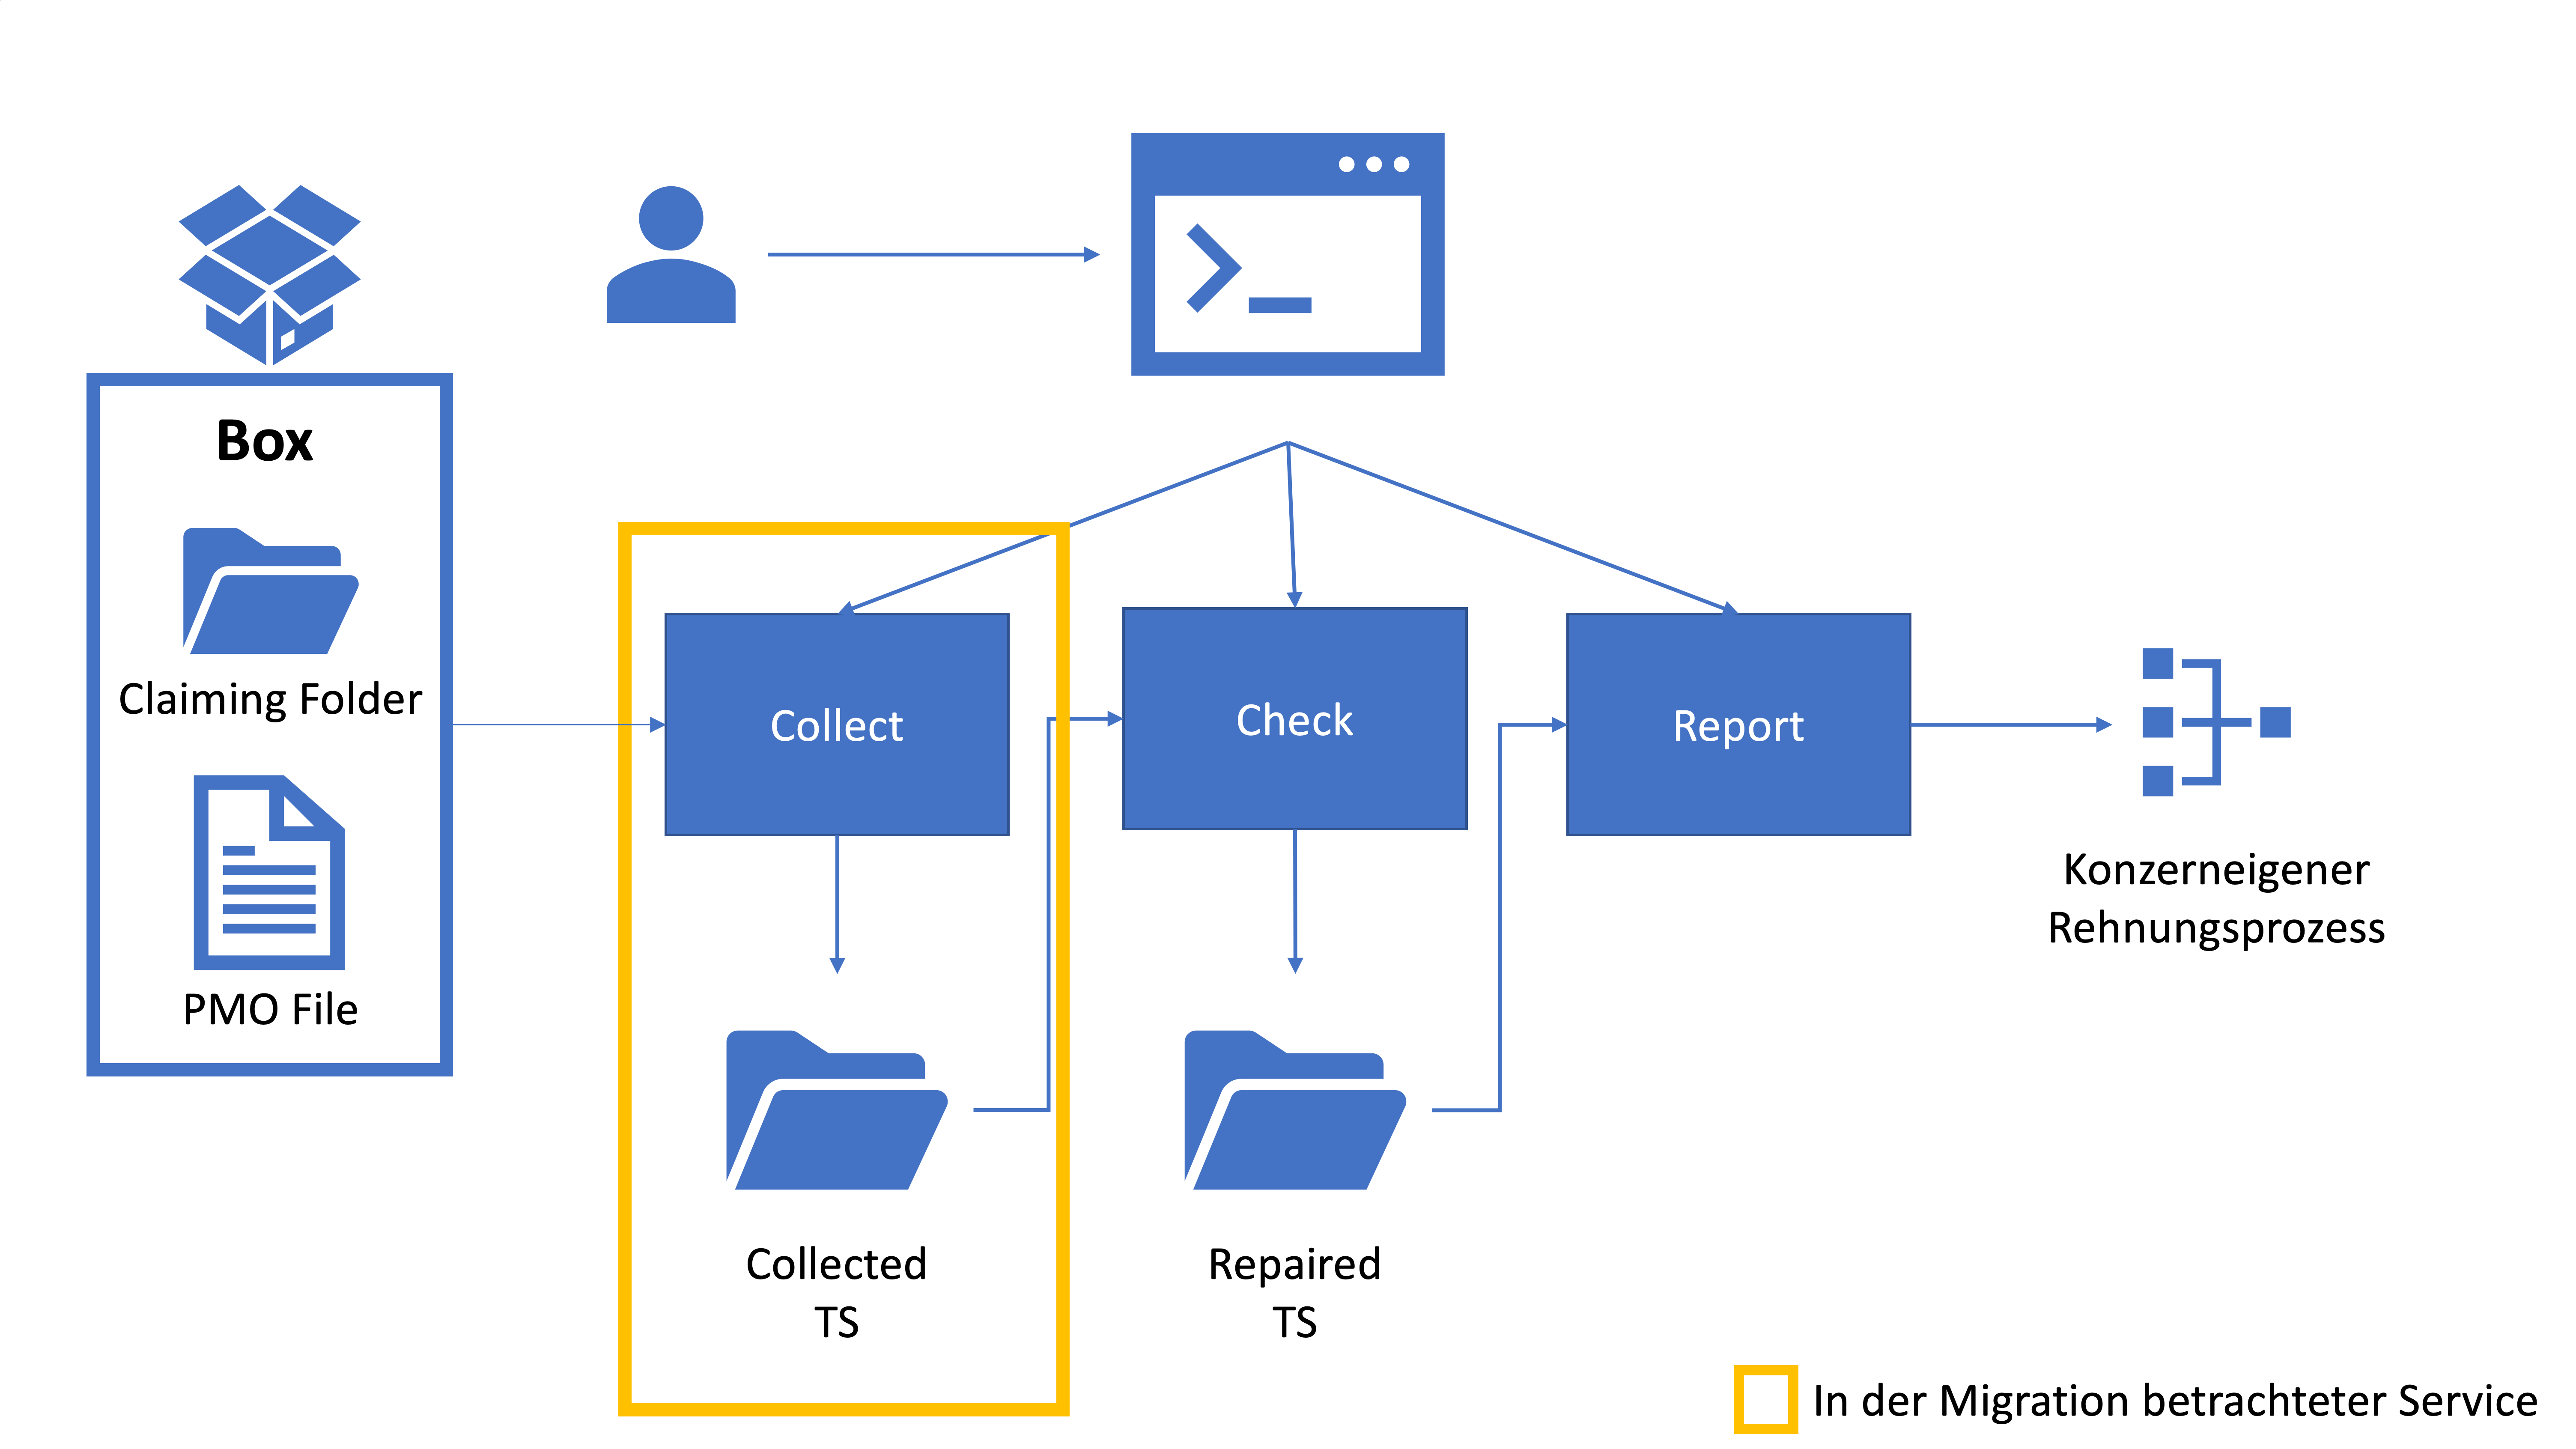
\includegraphics[width=0.65\textwidth]{pmo_python.png}
    \caption{Aufbau der ursprünglichen Anwendung (gelb umrandet der Teil, der prototypisch migriert wird)}
    \label{fig:pmo_python}
\end{figure}

Die bisher existierende Anwendung ist eine Python Anwendung, die grundsätzlich in dre Module aufgeteilt ist:
\begin{itemize}
\item \textbf{Timesheet Collector: }Einsammeln der Timesheets der in dem Projekt aktiven Mitarbeiter
\item \textbf{Timesheet Checker: }Überprüfen der Timesheets auf Korrektheit uns Vollständigkeit und gegebenenfalls Reparatur dieser
\item \textbf{Report Creator: }Erzeugung eines Reports und automatisierte Rechnungsstellung
\end{itemize}

Jeder dieser drei Services ist ein eigenes Python Modul. Diese greifen jeweils auf weitere Services wie einen Excel-Helper und Checking-Tools zurück.

Da es sich bei dieser Arbeit um eine Machbarkeitsstudie mit Erstellung eines Prototypen handelt, wird im ersten Schritt nur die Migration des Collect Service untersucht, bevor die anderen, komplexeren Services migriert werden. Dies ist in Abbildung \ref{fig:pmo_python} entsprechend durch den gelben Rahmen gekennzeichnet. Der Collect Service benötigt eine Verbindung zu dem Box-Verzeichnis und einen Ablageort für die \glqq{eingesammelten}\grqq{} Timesheets.

\subsection{Anforderungen an die Cloud Migration}
Wird eine Anwendung in die Cloud migriert werden unter anderem folgende Vorteile erwartet \cite[Vgl. auch im Folgenden][03:23-05:36min]{AWS2019}:
\begin{itemize}
\item Kostensenkung
\item Steigerung der Produktivität
\item Agilität in der Entwicklung
\end{itemize}

Darüber hinaus muss vor der Migration untersucht und festgelegt werden, welche der in Kapitel \ref{sec:migrationsansaetze} herausgearbeiteten Migrationsstrategien verfolgt werden soll \cite[Vgl.][10:38-13:23min]{AWS2019}. Jede dieser Strategien bietet ihre Vor- und Nachteile, weshalb diese Entscheidung individuell von der Anwendungsarchitektur und der Art der Benutzung abhängig ist. \pagebreak

Grundlegend kann der Migrationsprozess  in vier Schritte zusammengefasst werden \cite[Vgl. auch im Folgenden][S. 34f]{Maenhaut2016}:
\begin{enumerate}
\item \textbf{Auswahl der Komponenten:} Die Auswahl der zu migrierenden Komponenten sollte als erster Schritt vorgenommen werden. Wird die ganze Anwendung migriert ist dieser entsprechend einfach. Zu beachten ist hier vorallem die Kommunikation zwischen den Komponenten und damit verbundenen Sicherheitsanforderungen.
\item \textbf{Feststellen kompatibler Provider:} Verschiedene Provider bieten verschiedene Möglichkeiten und haben unterschiedliche limitierende Faktoren. Somit sollte ein Provider gefunden werden, der alle gewünschten Features abdecken kann.
\item \textbf{Einfluss auf das Client Netzwerk untersuchen:} Da die Kommunikation zwischen einzelnen Komponenten ins Internet verlagert wird, muss möglicher Weise die Bandbreite des Client Netzwerks angehoben werden.
\item \textbf{Skalierung der Anwendung:} Einer der Vorteile des Cloud Computing ist die Skalierbarkeit, also die Fähigkeit, bei großer Last weitere Instanzen einer Anwendung zu starten. Um diese Skalierbarkeit bereitstellen zu können müssen die Komponenten lokalisiert werden, die entsprechend angepasst werden müssten.
\end{enumerate}

Bei dem in dieser Arbeit untersuchten Prototypen werden alle Komponenten des Collect Service migriert, weshalb keine speziellen Komponenten ausgewählt werden müssen oder die Kommunikation zwischen diesen geprüft werden muss. Somit ist der erste Schritt recht einfach abzuschließen. Die Auswahl eines Passenden Providers wird im weiteren Verlauf dieser Arbeit beschrieben. Einen Einfluss auf das Client Netzwerk wird der Prototyp nicht haben, es sollte lediglich hinsichtlich der Auswahl des Cloud Providers darauf geachtet werden, dass die Netzwerkanbindung ausreicht um zum Beispiel das Projektmanagement-File zuverlässig herunterzuladen. Die Skalierbarkeit der Anwendung bleibt für den ersten Prototypen vorerst außerhalb der Zielsetzung, diese würde erst nach einer erfolgreichen Machbarkeitsstudie weiter betrachtet werden.

Darüber hinaus soll eine Anwendung in der Cloud je nach Bedarf auch von mehr Nutzern gleichzeitig nutzbar sein, weshalb auch über die Umsetzung von \textit{multi-tenancy} nachgedacht werden sollte \cite[Vgl.][S. 34ff]{Maenhaut2016}. Im Falle des in dieser Arbeit beschriebenen Prototypen ist das jedoch erst einmal nicht nötig.
\pagebreak
% Use-Case Analyse
\section{Use-Case Modellierung}
\label{sec:use-case-modellierung}

Nachfolgend wird die ursprüngliche Anwendung funktional Beschrieben, um daraus die Qualitätsanforderungen für die Migrierte Anwendung abzuleiten. Durch das Testen auf die Qualitätsanforderungen soll untersucht werden, ob sich eine Veränderung im Nutzungsverhalten bei der Migration in die Cloud ergibt.

\subsection{Funktionale Beschreibung der bisherigen Anwendung}
Die Funktionalität der bisherigen Anwendung besteht darin, den Prozess der Rechnungsstellung zu automatisieren und somit management Aufwände zu reduzieren. Dazu besteht die Anwendung hauptsächlich aus drei Services, dem \textit{Collect Service}, dem \textit{Check Service} und dem dem \textit{Report Service}. Ausgeführt wird die Anwendung bisher auf einem lokalen System und greift über das lokale Verzeichnis mithilfe einer \gls{Box}-Integration auf diese zu. Zur Ausführung der Anwendung wird eine Konfigurationsdatei benötigt, die alle notwendigen Pfade und Parameter enthält. In dem \gls{Box}-Verzeichnis liegen die \textit{\glspl{Timesheet}} der Mitarbeiter des Projektes und eine Projektmanagementdatei (PMO-File), die allgemeine Informationen zum Projekt und den Mitarbeitern enthält.

Aufgabe des \textit{Collect Service} ist es, aus dem PMO-File oder einer alternativen Mitarbeiterliste alle, aktuell in dem Projekt aktiven Mitarbeiter zu ermitteln und die \textit{\glspl{Timesheet}} dieser in ein \textit{Collect}-Verzeichnis zu kopieren. Der \textit{Check Service} gleicht die von den Mitarbeitern manuell ausgefüllten \textit{\glspl{Timesheet}} mit den Daten aus einem Zeiterfassungstool und ermittelt, ob die Daten korrekt sind oder gegebenenfalls korrigiert werden müssen. Abschließend werden im \textit{Report Service} aus den Daten die Rechnungen für den Kunden erstellt, indem die Informationen aus den \textit{\glspl{Timesheet}} detailliert auf die einzelnen Teilprojekten aufgeteilt und abgerechnet werden.

In dieser Arbeit soll untersucht werden, ob sich eine Veränderung im Nutzungsverhalten bei der Migration in die Cloud ergibt und ob die Business-Logik entsprechend angepasst werden muss. \pagebreak

\subsection{Wie könnte ein Cloud Setup Aussehen?}
Durch die Migration in die Cloud ergeben sich viele Möglichkeiten für die Anwendung. Unter anderem bringt die Cloud-Migration \textit{\gls{Multi-Tenancy}}, also eine Mehrbenutzerfähigkeit mit sich, damit die Anwendung von mehreren Nutzern gleichzeitig verwendet werden kann, ohne dass diese sich beeinflussen oder behindern.

Um die Anwendung allgemein in die Cloud zu migrieren, könnte diese so wie sie ist mit \textit{Lift-and-Shift} in eine virtuelle Maschine Kopiert werden und würde somit in der Cloud bereitgestellt. Dadurch könnte jedoch keine Aussage darüber getroffen werden, inwiefern die Anwendung oder ihre Architektur verändert werden muss, um die Vorteile einer Cloud-nativen Anwendung in der Cloud auszunutzen.

Aus diesem Grund soll die Anwendung zu einer Web-Anwendung weiterentwickelt werden. Dadurch verändert sich die Art und Weise, wie die Use-Cases Ausgeführt werden und wie die Anwendung benutzt wird. Diese Veränderungen werden am Beispiel der Migration des \textit{Collect Service} untersucht.

\subsection{Collect Service}
\textbf{Bisherige Verwendung:} Der für den Prototypen ausgewählte Use-Case ist das \glqq{Einsammeln}\grqq der \textit{\glspl{Timesheet}}. Aus einer Konfigurationsdatei hinaus soll festgelegt werden für welches Projekt und welchen Zeitraum diese von dem Projektverzeichnis in ein temporäres Verzeichnis kopiert werden sollen. 

\textbf{Möglichkeiten einer Web-Anwendung:} Durch die Migration in die Cloud und die Weiterentwicklung zu einer Web-Anwendung können die Funktionen der Anwendung zukünftig über einen API-Endpunkt bereitgestellt werden und die Ausführung dieser kann zum Beispiel nach einem Zeitplan oder einem Trigger, wie das Hochladen einer neuen Konfigurationsdatei erfolgen. Auf die hierzu notwendigen technischen Veränderungen wird später in der Arbeit eingegangen. \pagebreak

\textbf{Use-Case Definition:} Nachfolgend wird der Use-Case definiert, um im Anschluss an die Implementierung untersuchen zu können, ob dieser auch nach der Migration in die Cloud erfüllbar ist.

\begin{figure}[H]
    \centering
    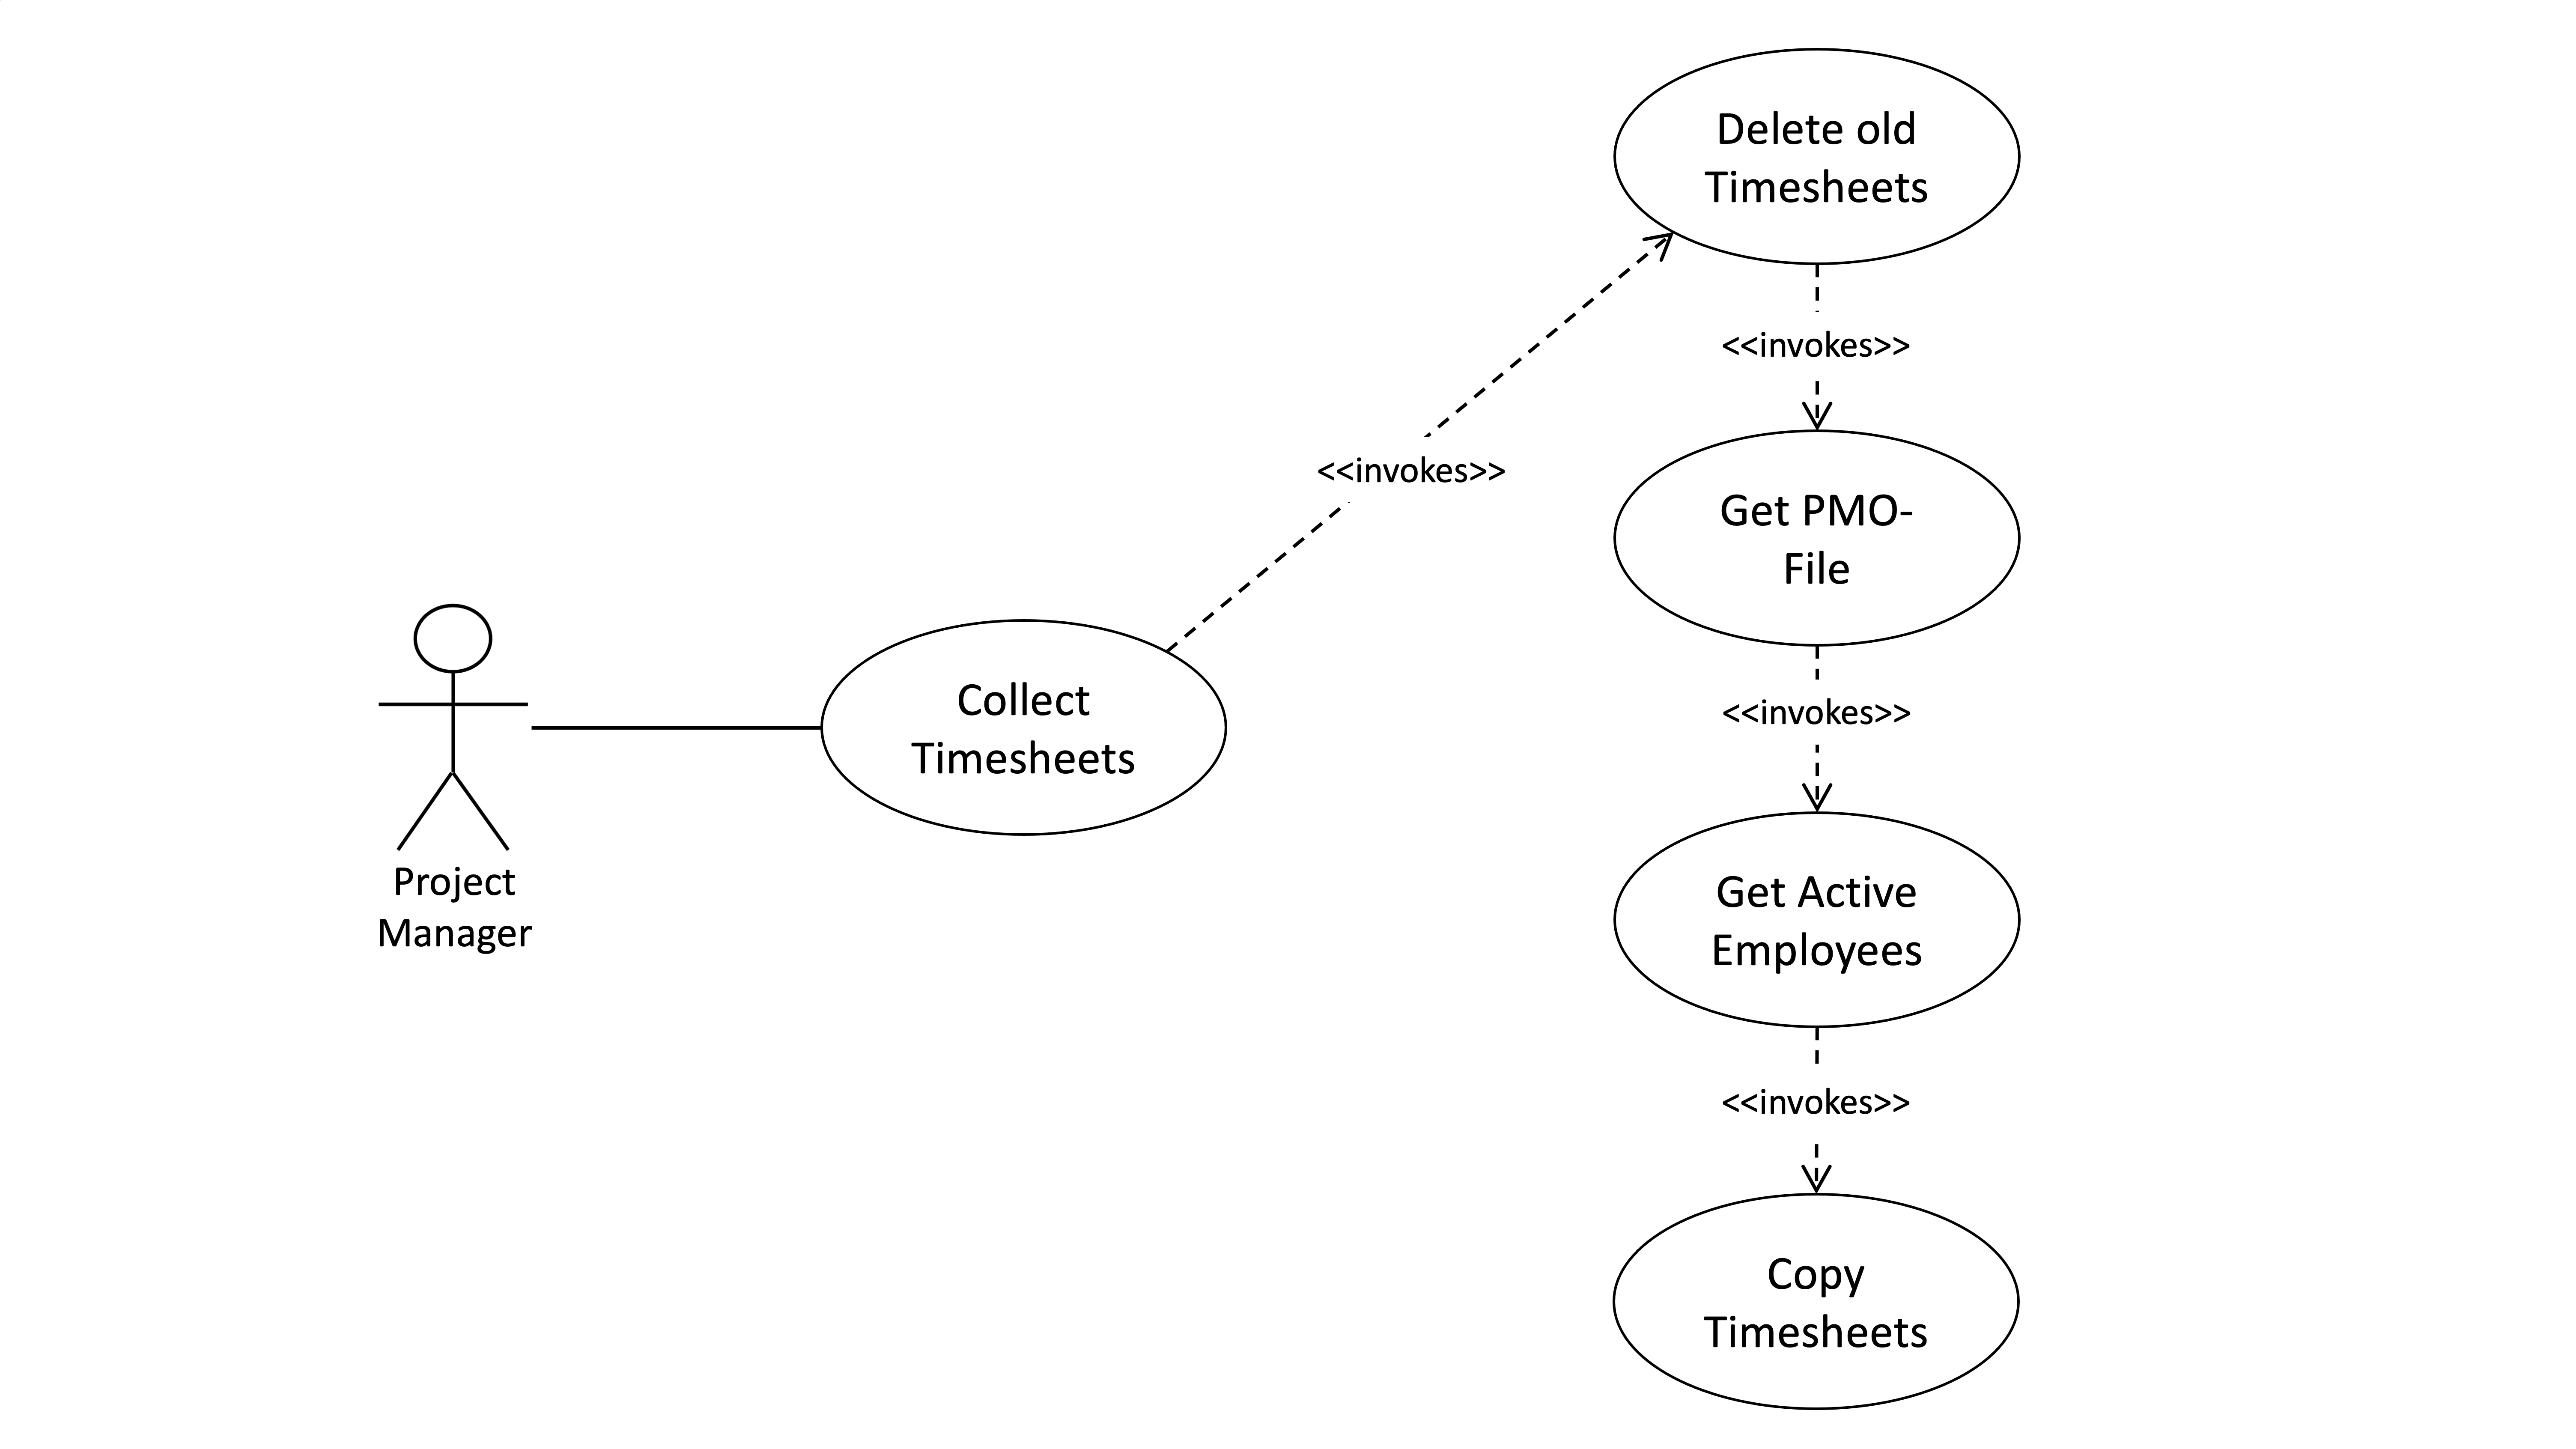
\includegraphics[width=\textwidth]{use-case-diagram.png}
    \caption{Use-Case Diagramm}
    \label{fig:use-case-diagram}
\end{figure}

Abbildung \ref{fig:use-case-diagram} stellt grafisch dar, welche Aufgaben der \textit{Collect Service} erfüllen muss und in welcher Reihenfolge diese ausgeführt werden. diese grundlegende Funktionsweise darf durch eine Cloud Migration nicht beeinträchtigt werden.

\begin{table}[H]
    \begin{tabular}[H]{|l|l|}
        \hline
        \multicolumn{2}{|l|}{\textbf{Anwendungsfall:} Einsammeln der \textit{\glspl{Timesheet}}} \\
        \hline
        \textbf{Kurzbeschreibung:} & \textit{\glspl{Timesheet}} aktiver Mitarbeiter in temporäres Verzeichnis kopieren \\
        \hline
        \multicolumn{2}{|l|}{\textbf{Normalverlauf}} \\
        \hline
        \multicolumn{2}{|l|}{1. Leeren des temporären Ordners} \\
        \multicolumn{2}{|l|}{2. PMO Datei finden und laden} \\
        \multicolumn{2}{|l|}{3. Aktive Mitarbeiter aus PMO Datei lesen} \\
        \multicolumn{2}{|l|}{4. \textit{\glspl{Timesheet}} der aktiven Mitarbeiter kopieren} \\
        \hline
        \multicolumn{2}{|l|}{\textbf{Alternativablauf}} \\
        \hline
        \multicolumn{2}{|l|}{Siehe Normalverlauf} \\
        \multicolumn{2}{|l|}{\textbf{Qualitätsanforderungen}} \\
        \hline
        \multicolumn{2}{|l|}{1. Für jeden aktiven Mitarbeiter soll ein \textit{\gls{Timesheet}}im temporären Ordner liegen} \\
        \multicolumn{2}{|l|}{2. Die \textit{\glspl{Timesheet}} sollen unverändert sein (Dateiname, Inhalt)} \\
        \multicolumn{2}{|l|}{3. Eigener Zielordner pro Monat zur Vermiedung von Vermischungen} \\
        \multicolumn{2}{|l|}{4. Die \textit{\gls{Timesheet}} Größe kann variieren -> keine Limitierungen} \\
        \multicolumn{2}{|l|}{5. Es darf keine Kompression mit Formatänderung eingesetz werden} \\
        \multicolumn{2}{|l|}{6. Ein Logfile soll Erfolg und Misserfolg von Kopiervorgängen enthalten} \\
        \multicolumn{2}{|l|}{7. Fehlersituationen auf einzelnen Dateien dürfen den Ablauf nicht unterbrechen} \\
        \multicolumn{2}{|l|}{8. Root-Verzeichnisse für Ziel und Quelle müssen konfigurierbar sein} \\
        \hline
    \end{tabular}
    \caption{Anwendungsfall: Einsammeln der \textit{\glspl{Timesheet}}}
    \label{tab:use-case-analyse-timesheets}
\end{table}

Anschließend an diesen Prozess würden die weiteren Services der Toolsuite folgen, die für den Umfang dieser Arbeit ausgelassen wurden.